\documentclass[letter,12pt,twoside]{hmcpset}
\usepackage[utf8]{inputenc}
\usepackage[english]{babel}
\usepackage{fancyhdr}
\usepackage[margin=1in]{geometry}
\usepackage{graphicx}
\usepackage{amsmath}
\usepackage{mathtools}
\usepackage[mathscr]{euscript}
\usepackage{lmodern} % math, rm, ss, tt
\usepackage[T1]{fontenc}
\usepackage{relsize}
\usepackage{tikz}
%\newcommand*{\ms}[1]{\ensuremath{\mathscr{#1}}}
\renewcommand{\labelenumi}{{\bf (\alph{enumi})}}

\pagestyle{fancy}
\fancyhf{}
\rhead{Spring 2019}
\lhead{\vspace{5mm} Math 147 Topology}
\rfoot{Page \thepage}
\chead{Section 8}
 
\renewcommand{\headrulewidth}{2pt}
\renewcommand{\footrulewidth}{2pt}

\graphicspath{ {./figures_theorems/} } 

% info for header block in upper right hand corner
\begin{document}
\section*{Chapter 8\\ Continuity: When Nearby Points Stay Together}

\begin{problem}[Theorem 8.1] 
    Let $X$ and $Y$ be topological spaces and let $f: X \rightarrow Y$ be 
    a function. Then the following are equivalent:
    \begin{enumerate}
        \item The function $f$ is continuous.
        \item For every closed set $K$ in $Y$, the inverse image 
        $f^{-1}(K)$ is closed in $X$.
        \item For every limit point $p$ of a set $A$ in $X$, the image 
        $f(p)$ belongs to $\overline{f(A)}$.
        \item For every $x \in X$ and open set $V$ containing $f(x)$, 
        there is an open set $U$ containing $x$ such that $f(U) \subset V$.
    \end{enumerate}
\end{problem}

\begin{proof}
    \begin{itemize}
        \item (1 $\iff$ 2). Observe firstly that we can write $f^{-1}(K) = X - f^{-1}(Y - K)$.
        This is because every $x \in f^{-1}(Y - K)$ will be mapped to $Y - K$. 
        Hence every $x \in X - f^{-1}(Y - K)$ will be mapped to $K$. Now observe
        that since $K$ is closed (open), $Y - K$ is open (closed), 
        so that $f^{-1}(Y - K)$ 
        is an open (a closed) set in $X$. Therefore, we see that 
        $X - f^{-1}(Y - K) = f^{-1}(K)$ is a closed (open) set, as desired.

        \begin{figure}[h!]
            \centering
            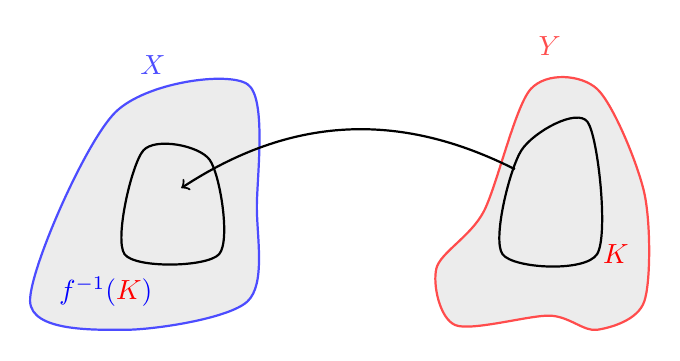
\begin{tikzpicture}[thick, scale = 1.2]
                \draw [red!70, fill = gray!15] plot [smooth cycle] coordinates {(5,0.25) (6,0.35)
                (6.5, 0.2) (7,0.5) (7,1.65) (6.5,2.75) (5.8,2.75)
                (5.3,1.45) (4.8,0.85) } node at (6,3.2) {$Y$}; 
    
                \draw [blue!70, fill = gray!15] plot [smooth cycle] coordinates
                {(1.5,.2)(2.8,.5)(2.9,1.5)(2.8,2.8)(1.4,2.5)(0.5,0.5)}
                node at (1.8,3) {$X$}; 
    
                \path[<-] (2.1, 1.7) edge [bend left] (5.63,1.9);
                x
                \draw [] plot [smooth cycle] coordinates {(1.5,1) (1.7, 2.1) (2.4,2) (2.5, 1)}
                node at (1.3, .6) {${\color{blue}f^{-1}({\color{red}K})}$};
    
                \draw plot [smooth cycle] coordinates {(5.5,1) (5.7, 2.1)
                (6.4,2.4) (6.5, 1)} node at (6.7, 1) {$\color{red}K$};
            \end{tikzpicture}
            \caption{Note: $f^{-1}$ may or may not be a function from $Y
            \to X$! This picture just demonstrates that for every closed
            $K \in Y$, $f^{-1}(K)$ is closed in $X$.
    }
        \end{figure}

        \item (1 $\implies$ 3) Suppose for the sake of contradiction that 
        $f(p)$ is an isolated point. Then there exists an open set $U$ of 
        $Y$ such that $f(p) \in U$ but $U \cap f(A) = \emptyset$. Now observe 
        that $f^{-1}(U)$ is open in $X$, and $p \in V$. But since $p$ 
        is a limit point of $A$, we know that $f^{-1}(U)$ must contain 
        some $q \ne p$
        and $q \in A$. However, this would imply that $f(q) \in U$, 
        which is a contradiction since we assumed that $U \cap f(A) =
        \emptyset$.
        Thus we see that $f(p) \in \overline{f(A)}$.

        \begin{figure}[h!]
            \centering
            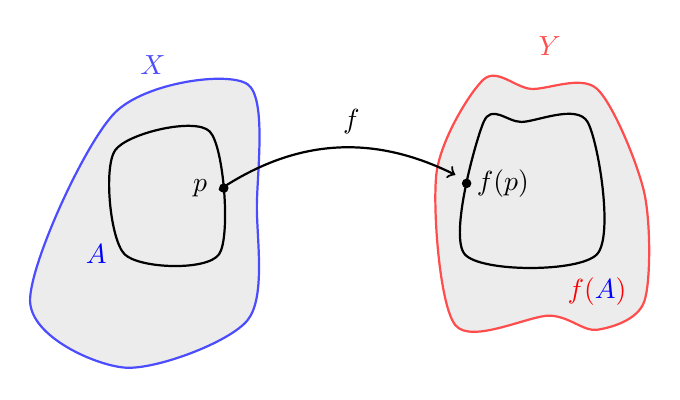
\begin{tikzpicture}[thick, scale = 1.2]
                \draw [red!70, fill = gray!15] plot [smooth cycle] coordinates {(5,0.25) (6,0.35)
                (6.5, 0.2) (7,0.5) (7,1.65) (6.5,2.75) (5.8,2.75)
                (5.3,2.85) (4.8,1.85) } node at (6,3.2) {$Y$}; 
    
                \draw [blue!70, fill = gray!15] plot [smooth cycle] coordinates
                {(1.5,-.2)(2.8,.3)(2.9,1.5)(2.8,2.8)(1.4,2.5)(0.5,0.5)}
                node at (1.8,3) {$X$}; 
    
                \path[->] (2.5, 1.68) edge [bend left] (5,1.84)
                node at (3.9, 2.4) {$f$};

                \draw [fill = black] (2.55, 1.7) circle (.25ex) node at
                (2.3, 1.7) {$p$}; 
                
                \draw [] plot [smooth cycle] coordinates {(1.5,1) (1.4, 2.1) (2.4,2.3) (2.5, 1)}
                node at (1.2, 1) {${\color{blue} A}$};
    
                \draw plot [smooth cycle] coordinates {(5.1,1) (5.3, 2.4) (5.7, 2.4)
                (6.4,2.4) (6.5, 1)} node at (6.5, .6) {$\color{red}f({\color{blue}A})$};

                \draw [fill = black] (5.12, 1.75) circle (.25ex)
                node[right] {$f(p)$}; 
            \end{tikzpicture}
            \caption{Here the limit point $p$ of $A$ maps to a
            limit point of $f(A)$.}
        \end{figure}

        \item (3 $\implies$ 1) To prove the other direction, suppose that $U$ 
        is open in $Y$. Then let $U = Y -\overline{f(A)}$ for some set $A \in X$. 
        Now by (3), we know that $f(\overline{A})
        = \overline{f(A)}$. Hence 
        $$
        f^{-1}(U) = f^{-1}(Y - \overline{f(A)}) = f^{-1}(Y - f(\overline{A}))
        $$
        maps 
        to $X - \overline{A}$, which is an open set. Thus for every open
        set $U \subset Y$, we have that $f^{-1}(U)$ is open so that $f$ is
        continuous.

        \item (1 $\implies$ 4) Suppose that $f(x)$ is contained in some open 
        $V \subset Y$ where $x \in X$. By definition of an open set, there 
        must exist some $U$ open in $Y$ such that $f(x) \in U \subset V$.
        Now observe that, by continuity, $f^{-1}(U)$ is some open set in $X$ 
        such that $x \in f^{-1}(U)$ and $f(f^{-1}(U)) = U \subset V$. Thus 
        there will always exist an open $W \in X$ such that $x \in W$ and 
        $f(W) \subset V$, as desired.
        \begin{figure}[h!]
            \centering
            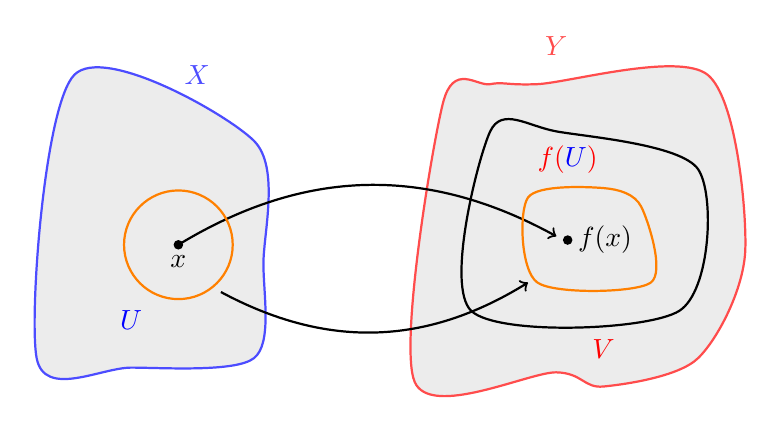
\begin{tikzpicture}[thick, scale = 1.2]
                \draw [red!70, fill = gray!15] plot [smooth cycle] coordinates {(4.5,0.25) (6,0.35)
                (6.5, 0.2) (7.5,0.5) (8,1.65) (7.6,3.5) (5.8,3.4)
                (5.3,3.4) (4.8,3.2) } node at (6,3.8) {$Y$}; 
    
                \draw [blue!70, fill = gray!15] plot [smooth cycle] coordinates
                {(1.5,.4)(2.8,.5)(2.9,1.5)(2.8,2.8)(0.9,3.5)(0.5,0.5)}
                node at (2.2,3.5) {$X$}; 
    
                \path[->] (2, 1.7) edge [bend left] (6, 1.79);

                \draw [fill = black] (2, 1.7) circle (.25ex) node[below] {$x$}; 
                
                \draw [orange] (2, 1.7) circle (3.8ex) node at (1.5, .9) {$\color{blue}U$}; 
    
                \draw plot [smooth cycle] coordinates {(5.1,1) (5.3, 2.9) (6, 2.9)
                (7.5,2.5) (7.3, 1)} node at (6.5, .6) {${\color{red}V}$};

                \draw [fill = black] (6.12, 1.75) circle (.25ex)
                node[right] {$f(x)$}; 

                \draw [orange] plot [smooth cycle] coordinates {(5.8, 1.3)
                (5.7, 2.2) (6.5, 2.3) (6.9, 2.1) (7, 1.3)} node at
                (6.12, 2.6)
                {$\color{red}f({\color{blue}U})$};

                \path[->] (2.45, 1.2) edge [bend right] (5.7, 1.3);

            \end{tikzpicture}
            \caption{In this diagram we see that a neighborhood $V$ of
            $f(x)$ corresponds to some open set $U$ of $x$ such that
            $f(U) \subset V$.}
        \end{figure}

        \item (4 $\implies$ 1) Consider an arbitrary open set $V$. By (4), we know 
        that for each $f(x) \in V$, there exists a $U$ open in $X$ such that 
        $f(U) \subset V$. Thus consider every $x \in X$ such that $f(x) \in V$, 
        and let $U_x$ be the open set in $X$ such that $f(U_x) \subset V$.
        Then observe that 
        $$
        \bigcup\limits_{x \in X \text{ s.t. } f(x) \in V}U_x = f^{-1}(V).
        $$
        This is because for any $x \in \bigcup\limits_{x \in X \text{ s.t. }
        f(x) \in V}U_x$, we know that $f(x) \notin Y - f(V)$ and for any 
        $y \in f(V)$, there exists a $x \in \bigcup\limits_{x \in X \text{ s.t.
        } f(x) \in V}U_x$ such that $f(x) = y$ by construction. Since the
        arbitrary union of open sets is open, we thus see that $f^{-1}(V)$ 
        is an open set. Since $V$ was an arbitrary open set, this proves that 
        $f$ is continuous by definition.
    \end{itemize}
\end{proof}

\begin{problem}[Theorem 8.2]
    Let $X$, $Y$ be topological spaces and $y_0 \in Y$. The constant map 
    $f : X \rightarrow Y$ defined by $f(x) = y_0$ is continuous.
\end{problem}

\begin{proof}
    We can use the fourth property of continuity to prove this assertion.
    Observe that if $V$ is any open set containing $y_0$, then $f^{-1}(V) = X$
    because $f(X) = y_0$, as $f$ is the constant map. If $V$ is an open 
    set not containing $y_0$, then $f^{-1}(V) = \emptyset.$ Since $X$,
    $\emptyset$
    are open, we have that the inverses of open sets in $Y$ are open sets in
    $X$. Therefore, $f$ is a continuous mapping. 
\end{proof}

\begin{problem}[Theorem 8.3]
    Let $X \subset Y$ be topological spaces. The inclusion map $i : X
    \rightarrow Y$ defined by $i(x) = x$ is continuous.
\end{problem}

\begin{proof}
    Observe that since if $U$ is open in $X \subset Y$, then $i^{-1}(U) = U$
    is open in $X$. Thus by the definition of continuity, we see that $i(x)$ 
    is a continuous mapping.
\end{proof}

\begin{problem}[Theorem 8.4]
    Let $f: X \rightarrow Y$ be a continuous map between topological spaces,
    and let $A$ be a subset of $X$. Then the restriction map 
    $f|_A : A \rightarrow Y$ defined by $f|_A(a) = f(a)$ is continuous.    
\end{problem}

\begin{proof}
    Consider $a \in A \subset X$ and an open set $V$ containing $f(a)$. Then 
    there is an open set $U$ of $X$ containing $a$ such that $f(U) \subset V$.
    Now observe that in the subspace topology, $A \cap U$ is an open set in 
    $A$. Furthermore, $f(A \cap U) \subset V$, since $A \cap U \subset U$.
    Therefore, we see that for every $a \in A$ and open set $V$ containing
    $f(a)$, there is an open set $A \cap U$ of $A$ containing $a$ such that $f(A
    \cap U) \subset V$, so that $f|_A: A \rightarrow Y$ is a continuous mapping.
\end{proof}

\begin{problem}[Theorem 8.5]
    A function $f: \mathbb{R}_{\text{std}} \rightarrow \mathbb{R}_{\text{std}}$
    is continuous if and only if for every $x \in \mathbb{R}$ and $\epsilon >
    0$, there is a $\delta > 0$ such that for every $y \in \mathbb{R}$ with 
    $d(x, y) < \delta$, then $d(f(x), f(y)) < \epsilon$.
\end{problem}

\begin{proof}
    First we'll prove the forward direction. Suppose that $f$ is a continuous
    function from $\mathbb{R}_{\text{std}} \rightarrow \mathbb{R}_{\text{std}}$.
    By using the fourth property of continuous functions, we know that for every
    $x \in \mathbb{R}$ and open set $V$ containing $f(x)$, there is an open set 
    $U$ containing $x$ such that $f(U) \subset V$. 
    \\
    \\
    Since the basis for
    $\mathbb{R}_\text{std}$ consists of balls, we can let $V = B(f(x),
    \epsilon)$. Now we can take $U$ to be a ball $B(x, \delta)$ such that 
    for every $y \in B(x, \delta)$ we have that $f(y) \in B(f(x, \epsilon))$.
    In terms of the metric space, this means that the continuity of $f$ implies 
    that for every $\epsilon > 0$, there must be a $\delta > 0$ such that 
    $d(x, y) < \delta \implies d(f(x), f(y)) < \epsilon$, which is the calculus
    definition of continuity.
    \\
    \\
    Now we prove the other direction. Observe that if the calculus definition of
    continuity is given, then we can see that the freedom granted to $\epsilon >
    0$ allows $d(f(x), y) < \epsilon$ to specify any arbitrary neighborhood
    $V$ in $\mathbb{R}$ which contains $f(x)$, where $x \in \mathbb{R}$.
    Now the fact that we know there exists a $\delta > 0$ such that 
    $d(x, y) < \delta \implies d(f(x), f(y)) < \epsilon$ implies the existence
    of an open set $U$ containing $x$ such that $f(U) \subset V$. This is exactly
    the fourth property of continuity offered in Theorem 8.1, which allows us to
    conclude that $f$ is a continuous mapping, as desired.
\end{proof}
\textbf{\emph{Q} (3/13/19)}: Is first countability necessary for the forward direction?\\
\begin{problem}[Theorem 8.6]
    Let $X$ be a $1^{\text{st}}$ countable space and $Y$ a topological space.
    Then a function $f: X \rightarrow Y$ is continuous if  and only if for 
    each convergent sequence $x_n \rightarrow x$ in $X$, $f(x_n)$
    converges to $f(x)$ in $Y$.
\end{problem}

\begin{proof}   
    First we prove the forward direction. Suppose that $f$ is a continuous
    mapping, $X$ is $1^{\text{st}}$ countable, and there is a sequence in $X$
    such that $x_n \rightarrow x$.
    \\
    \\
    Consider an open set $V$ in $Y$ such that $f(x) \in V$. Since $f$ 
    is continuous, $U = f^{-1}(V)$ is an open set in $X$. Therefore there 
    exists some $N \in \mathbb{N}$ such that for $i > N$, $x_i \in U$.
    Applying $f$ to this last equation implies that $f(x_i) \in f(U)
    = f(f^{-1}(V)) = V$. Thus by definition, $f(x_i)$ is a sequence which 
    converges to $f(x)$ in $Y$.
    \\
    \\
    Next we prove the other direction. Suppose $x_n \rightarrow x$
    and $f(x_n) \rightarrow f(x)$. For the sake of contradiction, suppose 
    $f$ is not continuous. By property (3) of Theorem 8.1, for some $A \subset
    X$ there exists a $p \in \overline{A}$ such that $f(p) \notin
    f(\overline{A})$.
    \\
    \\
    Since $f$ is first countable, we know by Theorem 6.18 that 
    there exists a sequence $\{a_i\}_{i \in \mathbb{N}}$ of 
    points in $A$ such that $a_i \rightarrow p$. Since $a_i$ are points
    of $A$, we know that $f(a_i) \in f(A)$ for all $i \in \mathbb{N}$. 
    However, we also know that $f(p) \notin f(\overline{A})$, so that it 
    could not be the case that $f(a_i) \rightarrow f(p)$. However, 
    this is a contradiction, namely to our assumption. Therefore we must 
    have that $f$ is continuous. 
    
\end{proof}

\begin{problem}[Theorem 8.7]
    Let $X$ by a space with a dense set $D$, and let $Y$ be Hausdorff. Let 
    $f: X \rightarrow Y$ and $g: X \rightarrow Y$ be continuous functions such 
    that for every $d \in D$, $f(d) = g(d).$ Then for all $x \in X$, $f(x) = g(x).$    
\end{problem}

\begin{proof}
    Suppose that $f(x) \ne g(x)$ for some $x \notin D$. Since the points are
    distinct, and since $Y$ is Hausdorff, there must exist disjoint open sets 
    $U, V$ in $Y$ such that $f(x) \in U$ and $g(x) \in V$. Since both $f, g$ are
    continuous, there must exist open sets $U', V'$ in $X$ such that 
    $f(U') \subset U$ and $g(V') \subset V$. However, since $D$ is dense in $X$,
    both $U'$ and $V'$ must intersect with some portion of $D$; that is, 
    there is some $y \in U'$ and $z \in V'$ such that $y, z \in D$. Therefore, 
    we see that $f(y) \in U$ and $g(z) \in V$. But we know that by definition of
    the function, $f(y) = g(z)$, which contradicts the fact that $U \cap V =
    \emptyset.$ Therefore, we have a contradiction and it must be the case that 
    $f(x) = g(x)$ for all $x \in X$, as desired.
\end{proof}

\begin{problem}[Theorem 8.9]
    If $f : X \rightarrow Y$ and $g : Y \rightarrow Z$ are continuous 
    then their composition $g \circ f : X \rightarrow Z$. 
\end{problem}

\begin{proof}
    Consider an open set $V$ in $Z$. Since $g$ is continuous, we know that 
    $g^{-1}(V)$ is open in $Y$. Since $f$ is continuous, we also know that 
    $f^{-1}(g^{-1}(V))$ is open in $X$. That is $(g \circ f)^{-1}(V)$ is 
    open in $X$. Thus by definition $g \circ f$ is a continuous mapping.
\end{proof}
\noindent
\textbf{Presented in class on 3/13/19}

\begin{problem}[Theorem 8.10]
    (pasting lemma) Let $X = A \cup B$. where $A, B$ are closed in $X$. Let
    $f : A \rightarrow Y$ and $g : B \rightarrow Y$ be continuous funtions that 
    agree on $A \cap B$. Then the function $h :A\cup B \rightarrow Y$ 
    such that $h = f$ on $A$ and $h = g$ on $B$ is continuous.
\end{problem}

\begin{proof}
    Consider $K$ closed in $Y$. Then observe that $h^{-1}(K) = f^{-1}(K)
    \cup g^{-1}(K)$ is a union of closed sets in $A \cup B$. Thus 
    the union is itself closed, so that for every $K$ closed in $Y$ 
    we have that $h^{-1}(K)$ is closed in $A\cup B$, proving continuity.    
\end{proof}

\noindent
\textbf{Presented in class on 3/13/19}\\
\begin{problem}[Theorem 8.11]
    (pasting lemma) Let $X = A \cup B$. where $A, B$ are open in $X$. Let
    $f : A \rightarrow Y$ and $g : B \rightarrow Y$ be continuous funtions that 
    agree on $A \cap B$. Then the function $h :A\cup B \rightarrow Y$ 
    such that $h = f$ on $A$ and $h = g$ on $B$ is continuous.
\end{problem}

\begin{proof}
    Consider $K$ open in $Y$. Then observe that $h^{-1}(K) = f^{-1}(K)
    \cup g^{-1}(K)$ is a union of open  sets in $A \cup B$. Thus 
    the union is itself open, so that for every $K$ open in $Y$ we have 
    that 
    $h^{-1}(K)$ is open in $A\cup B$, proving continuity.   
\end{proof}

\begin{exercise}[Exercise 8.12]
\textbf{Exercise 8.12} Is the pasting lemma true when $A$ and $B$ in
the preceeding theorems are arbitrary sets?
\end{exercise}

\begin{solution}
The answer is no, since $A \cap B$ may turn out to be neither an open
or closed set. Based on the definition $h : A \cup B \to Y$, it is
possible that $h$ would experience a discontinuity in transitioning
from $A$ to $A \cap B$ or $B$ to $A \cap B$. 
\end{solution}

\begin{problem}[Theorem 8.13] Let $f: X \rightarrow Y$ be a function
and $\mathscr{B}$ a basis for $Y$. Then $f$ is continuous if and only
if for every open set $B$ in $\mathscr{B}$, $f^{-1}(B)$ is open in $X$.
\end{problem}

\begin{proof}
    First we'll prove the forward direction. Suppose $f$ is
    continuous. If $\mathscr{B} = \{B_\alpha : \alpha \in \lambda\}$
    is a basis for $Y$, then observe that for every $\alpha \in
    \lambda$, $f^{-1}(B_\alpha)$ is an open set in $X$ by the
    continuity of $f$, which proves this direction. 
    \\
    \\
    Next we prove the other direction. Suppose $\mathscr{B}$ is a
    basis for $Y$ and for every $B \in \mathscr{B}$, $f^{-1}(B)$ is
    open in $X$. Then if $V$ is open in $Y$, observe that 
    \[
        f^{-1}(V) = f^{-1}(\bigcup\limits_{\alpha \in \lambda} B_\alpha) = 
        \bigcup\limits_{\alpha \in \lambda}f^{-1}(B_\alpha) 
    \]
    Since $f^{-1}(V)$ is a union of open sets in $X$, we have that
    $f^{-1}(V)$ is open in $X$. Since this holds for all $V$ open in
    $Y$, we have that $f$ is continuous.
\end{proof}

\begin{problem}[Theorem 8.14] Let $f: X \rightarrow Y$ be a function
and $\mathscr{B}$ a subbasis for $Y$. Then $f$ is continuous if and only
if for every open set $B$ in $\mathscr{B}$, $f^{-1}(B)$ is open in $X$.
\end{problem}

\begin{proof}
    First we'll prove the forward direction. Suppose $f$ is
    continuous. If $\mathscr{B} = \{B_\alpha : \alpha \in \lambda\}$
    is a basis for $Y$, then observe that for every $\alpha \in
    \lambda$, $f^{-1}(B_\alpha)$ is an open set in $X$ by the
    continuity of $f$, which proves this direction. 
    \\
    \\
    Next we prove the other direction. Let $x \in X$ and suppose
    $V$ is an open set in $Y$ containing $f(x)$. Since $\mathscr{B}$ 
    is a subbasis for $Y$, there must exists a
    finite set $\{B_i\}_{i = 1}^n \subset \mathscr{B}$ such that
    $\bigcap\limits_{i = 1}^nB_i \subset V$. Therefore, 
    \[
      f^{-1}(V) \supset f^{-1}(\bigcap\limits_{i = 1}^nB_i) = \bigcap\limits_{i = 1}^n f^{-1}(B_i) = U.
    \]  
    where we have denoted $U = \bigcap\limits_{i = 1}^n f^{-1}(B_i)$. 
    Since this is a finite intersection of open sets, each which
    contain $x$, we have that $U \subset f^{-1}(V)$. By property (3)
    of Theorem 8.1, we have that $f$ is continuous as desired.
\end{proof}

\begin{problem}[Theorem 8.15]
    If $X$ is compact and $f: X \rightarrow Y$ is continuous and 
    surjective, then $Y$ is compact.
\end{problem}

\begin{proof}
    Consider an open cover $\mathscr{U} = \{U_\alpha : \alpha \in
    \lambda\}$ of $Y$. Since $f$ is continuous, 
    $f^{-1}(U_\alpha)$
    is open in $X$ for all $\alpha \in \lambda$.
    Since $Y$ is closed in $Y$,
    $f^{-1}(Y)$ is a closed subspace in $X$. By theorem 7.8,
    $f^{-1}(Y)$ is therefore compact. Since 
    $\{f^{-1}(U_\alpha) : \alpha \in 
    \lambda\}$ is an open cover of $f^{-1}(Y)$ there exists a finite
    subcover, denoted as $\{f^{-1}(U_1), \dots, f^{-1}(U_n)\}$. 
    \\
    \\
    Since 
    \[
        f^{-1}(Y) \subset \bigcup\limits_{i = 1}^n f^{-1}(U_n) \implies 
        Y \subset f(\bigcup\limits_{i = 1}^n f^{-1}(U_n))
        = \bigcup\limits_{i = 1}^n f(f^{-1}(U_n)) 
        = \bigcup\limits_{i = 1}^n U_n.
    \]
    Thus we have that $\{U_1, \dots , U_n\}$ is a finite subcover of 
    $\mathscr{U}.$ Since $\mathscr{U}$ was an arbitrary open cover,
    this proves that $Y$ is compact.

    \begin{figure}[h!]
        \centering
        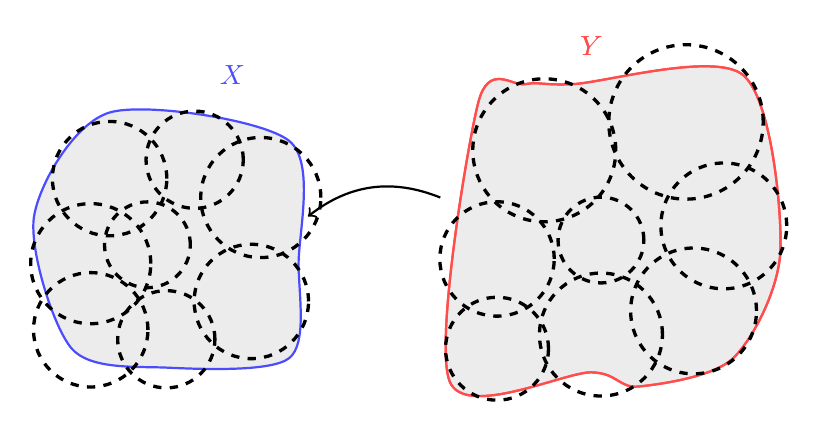
\begin{tikzpicture}[thick, scale = 1.2]
            \draw [red!70, fill = gray!15] plot [smooth cycle] coordinates {(4.5,0.25) (6,0.35)
            (6.5, 0.2) (7.5,0.5) (8,1.65) (7.6,3.5) (5.8,3.4)
            (5.3,3.4) (4.8,3.2) } node at (6,3.8) {$Y$}; 

            \draw [red!70] plot [smooth cycle] coordinates {(4.5,0.25) (6,0.35)
            (6.5, 0.2) (7.5,0.5) (8,1.65) (7.6,3.5) (5.8,3.4)
            (5.3,3.4) (4.8,3.2) } node at (6,3.8) {$Y$}; 

            \draw [blue!70, fill = gray!15] plot [smooth cycle] coordinates
            {(1.5,.4)(2.8,.5)(2.9,1.5)(2.8,2.8)(0.9,3.1)(0.1, 2)(0.5,0.6)}
            node at (2.2,3.5) {$X$}; 

            \draw [very thick, dashed] (2.4, 1.1) circle (4ex);
            \draw [very thick, dashed] (.9, 2.4) circle (4ex);
            \draw [very thick, dashed] (1.8, 2.6) circle (3.4ex);
            \draw [very thick, dashed] (2.5, 2.2) circle (4.2ex);
            \draw [very thick, dashed] (1.3, 1.7) circle (3ex);
            \draw [very thick, dashed] (.7, 1.5) circle (4.2ex);
            \draw [very thick, dashed] (.7, .8) circle (4ex);
            \draw [very thick, dashed] (1.5, .7) circle (3.4ex);

            \draw [very thick, dashed] (5, 1.55) circle (4ex);
            \draw [very thick, dashed] (5, 0.6) circle (3.6ex);
            \draw [very thick, dashed] (6.1, .75) circle (4.3ex);
            \draw [very thick, dashed] (6.1, 1.75) circle (3ex);
            \draw [very thick, dashed] (7.4, 1.9) circle (4.4ex);
            \draw [very thick, dashed] (7.08, 1) circle (4.4ex);
            \draw [very thick, dashed] (5.5, 2.7) circle (5ex);
            \draw [very thick, dashed] (7, 3) circle (5.4ex);

            % \draw plot [smooth cycle] coordinates {(5.1,1) (5.3, 2.9) (6, 2.9)
            % (7.5,2.5) (7.3, 1)} node at (6.5, .6) {${\color{red}V}$};

            % \draw [fill = black] (6.12, 1.75) circle (.25ex)
            % node[right] {$f(x)$}; 

            % \draw [orange] plot [smooth cycle] coordinates {(5.8, 1.3)
            % (5.7, 2.2) (6.5, 2.3) (6.9, 2.1) (7, 1.3)} node at
            % (6.12, 2.6)
            % {$\color{red}f({\color{blue}U})$};

            \path[<-] (3, 2) edge [bend left] (4.4, 2.2);
        \end{tikzpicture}
        \hspace{1cm}
        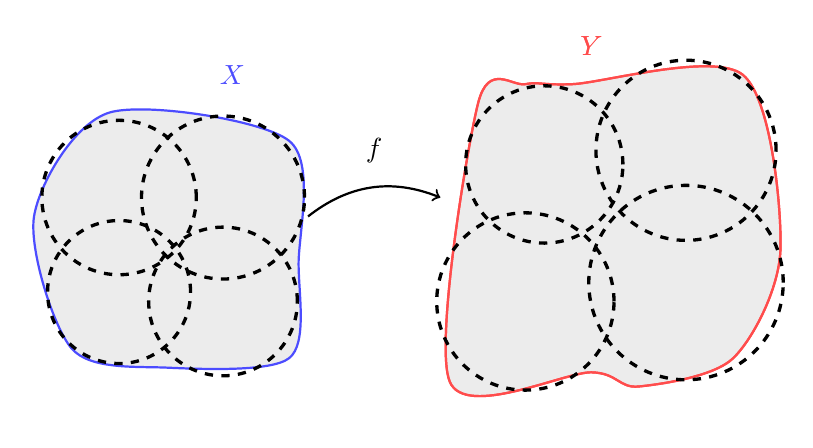
\begin{tikzpicture}[thick, scale = 1.2]
            \draw [red!70, fill = gray!15] plot [smooth cycle] coordinates {(4.5,0.25) (6,0.35)
            (6.5, 0.2) (7.5,0.5) (8,1.65) (7.6,3.5) (5.8,3.4)
            (5.3,3.4) (4.8,3.2) } node at (6,3.8) {$Y$}; 

            \draw [red!70] plot [smooth cycle] coordinates {(4.5,0.25) (6,0.35)
            (6.5, 0.2) (7.5,0.5) (8,1.65) (7.6,3.5) (5.8,3.4)
            (5.3,3.4) (4.8,3.2) } node at (6,3.8) {$Y$}; 

            \draw [blue!70, fill = gray!15] plot [smooth cycle] coordinates
            {(1.5,.4)(2.8,.5)(2.9,1.5)(2.8,2.8)(0.9,3.1)(0.1, 2)(0.5,0.6)}
            node at (2.2,3.5) {$X$}; 

            \draw [very thick, dashed] (2.1, 1.1) circle (5.2ex);
            \draw [very thick, dashed] (1, 1.2) circle (5ex);
            \draw [very thick, dashed] (1, 2.2) circle (5.4ex);
            \draw [very thick, dashed] (2.1, 2.2) circle (5.7ex);


            \draw [very thick, dashed] (5.5, 2.55) circle (5.5ex);
            \draw [very thick, dashed] (5.3, 1.1) circle (6.2ex);
            \draw [very thick, dashed] (7.0, 1.3) circle (6.8ex);
            \draw [very thick, dashed] (7, 2.7) circle (6.3ex);

            \path[->] (3, 2) edge [bend left] (4.4, 2.2) node at 
            (3.7, 2.7) {$f$};
        \end{tikzpicture}
        \caption{In the first diagram we 
        start with an arbitrary cover of $Y$, and take the
        inverse open images in $X$. In the second diagram, we identify
        finite subcover, which exists since $X$ is compact, and send
        this back into $Y$ to obtain a finite subcover of $Y$. }
    \end{figure}
\end{proof}

\begin{problem}[Theorem 8.18]
    Let $D$ be a dense subset of a topological space $X$ and let $f:X
    \rightarrow Y$ be continuous and surjective. Then 
    $f(D)$ is dense in $Y$.
\end{problem}

\begin{proof}
    Since $f$ is surjective, we have that $f(X) = Y$. Now observe that
    \[
      \overline{f(D)} = f(\overline{D}) = f(X) = Y  
    \]
    by property (3) of Theorem 8.1. Thus we have that $f(D)$ is dense
    in $Y$ as desired.
\end{proof}

\begin{problem}[Corollary 8.19]
    Let $X$ be as separable space and let $f: X \rightarrow Y$ be
    continuous and surjective. Then $Y$ is separable.
\end{problem}

\begin{proof}
    Since $X$ is separable there exists a countable dense set $A$ in
    $X$. Now observe that (1) $f(A)$ is at most countable since $f$ is
    surjective and (2) $f(A)$ is also dense in $Y$ by Theorem 8.18.
    Thus $Y$ also has a countable dense subset so $Y$ is separable.
\end{proof}

\noindent
\textbf{Exercise 8.20}
\begin{itemize}
    \item[1.] Find an open function that is not continuous. 
    \item[2.] Find a closed function that is not continuous.
    \item[3.] Find a continuous function that is neither open nor closed.
    \item[4.] Find a continuous function that is open but not closed.
    \item[5.] Find a continuous function that is closed but not open. 
\end{itemize}

\noindent
\textbf{Presented in class 3/25/19}\\
\begin{problem}[Theorem 8.21]
    If $X$ is normal and $f: X \rightarrow Y$ is continuous,
    surjective, and closed, then $Y$ is normal.
\end{problem}

\begin{proof}
    Consider two disjoint closed sets $A$ and $B$ in $Y$. By
    continuity, $f^{-1}(A)$ and $f^{-1}(B)$ must be closed sets in
    $X$. As they are disjoint, and because $X$ is normal,
    there must exist disjoint open sets $U$
    and $V$ such that $f^{-1}(A) \subset U$ and $f^{-1}(B) \subset V$.
    \\
    \\
    Observe that $U^c, V^c$ are closed sets in $X$. By closedness of
    $f$, we know that $f(U^c), f(V^c)$ are closed sets in $Y$. Thus
    $f(U^c)^c = f(U)$ and $f(V^c)^c = f(V)$ are both open sets. Since
    $A \subset f(U)$ and $B \subset f(V)$, and $f(U)$ and $f(V)$ are
    disjoint as $U, V$ are disjoint, we have that $Y$ must be normal
    as desired.


\end{proof}

\begin{problem}[Theorem 8.22]
    If $\{B_\alpha : \alpha \in \lambda\}$ is a basis for $X$ and $f:
    X \rightarrow Y$ is continuous, surjective and open, then
    $\{f(B_\alpha)\}_{\alpha \in \lambda}$ is a basis for $Y$.
\end{problem}

\begin{proof}
    Suppose $V$ is an open set in $Y$ and $f(x) \subset V$ where $x
    \in X$. By continuity, there exists an open set $U \subset X$ such
    that $f(U) \subset V$. As $\{B_\alpha : \alpha \in \lambda\}$ is a
    basis for $X$, there exists a $B \in \{B_\alpha : \alpha \in
    \lambda\}$ such that $x \in B \subset U$ by Theorem 4.1.
    Therefore, $f(x) \in f(B) \subset V$. 
    \\
    \\
    Thus observe that 
    \begin{enumerate}
        \item 
        $\{f(B_\alpha)_{\alpha \in \lambda}\} \subset \mathscr{T}_Y$
        since by openness of $f$ each $f(B_\alpha)$ is open in $Y$ for all
        $\alpha \in \lambda$ and 
        
        \item for each open $V$ in $Y$ where $f(x)
        \in V$, there exists a $B \in
        \{B_\alpha : \alpha \in \lambda\}$ such that
        \[
            f(x) \in f(B) \subset V.
        \]
        \end{enumerate}
        As this satisfies Theorem 4.1, we have that
        $\{f(B_\alpha)\}_{\alpha \in \lambda}$ is a basis for $Y$.
    \end{proof}

\begin{problem}[Theorem 8.24]
    Let $X$ be compact and $Y$ be Hausdorff. Then any continuous
    function $f : X \rightarrow Y$ is closed. 
\end{problem}

\begin{proof}
    Let $A$ be a closed in $X$ and consider $y \in Y - f(A)$. 
    Let $\{U_\alpha\}_{\alpha \in \lambda}$ be an open cover of 
    $f(A)$ where $\lambda$ is an arbitrary index.
    \\
    \\
    By continuity, we know that each $f^{-1}(U_\alpha)$ is open so
    \[
        \{f^{-1}(U_\alpha)\}_{\alpha \in \lambda}
    \] 
    is an open cover of $A$ in $X$.
    By Theorem 7.8, we know that $A$ must be compact since it is a
    closed subspace of $X$, which is compact. Therefore, there exists
    a finite subcover of $\{f^{-1}(U_\alpha)\}_{\alpha \in \lambda}$, which we can
    denote as 
    \[
        \{f^{-1}(U_{\alpha_1}), \dots , f^{-1}(U_{\alpha_n})\}.
    \]
    Thus we know that $\{U_{\alpha_1}, \dots, U_{\alpha_n}\}$. is an open cover
    of $f(A)$. Since every open cover of $f(A)$ has a finite subcover,
    we can conclude that $f(A)$ is compact. By Theorem 7.9, we have
    that  $f(A)$ is closed since $f(A)$ is a compact subspace of $Y$ which is a Hausdorff
    space. Therefore, $f$ is a closed function.


\end{proof}

\begin{problem}[Theorem 8.25]
    Being homeomorphic is an equivalence relation on topological
    spaces. 
\end{problem}

\begin{proof}
    Let $X \sim Y$ if $X$ is homeomorphic to $Y$. 
    \\
    \\
    \textbf{Reflexive}: Observe that $X \sim X$ since the identity function $f$
    is a continuous bijective function with a continuous inverse. Thus
    $\sim$ is reflexive. 
    \\
    \\
    \textbf{Symmetric}: If $X \sim Y$, there exsits a continuous bijective
    function $f : X \rightarrow Y$ with a continuous inverse.
    Observe that $f^{-1} : Y \rightarrow X$ is also a continuous bijective
    function with a continuous inverse, so that $X \sim Y \implies Y
    \sim X$. Thus $\sim$ is symmetric.
    \\
    \\
    \textbf{Transitive}: 
    If $X \sim Y$ and $Y \sim Z$, where $f: X \rightarrow Y$ and $g :
    Y \rightarrow Z$ are continuous bijective functions with
    continuous inverses, then obseve that $g \circ f$ is a continous
    bijective function (we proved earlier that compositions of
    continuous functions are continuious, and bijectivity is
    immediate)
    and that $(g \circ f)^{-1}$ is a also continuous since the
    inverses $f^{-1}$ and $g^{-1}$ are both continuous. Since $g \circ
    f : X \rightarrow Z$, we see that $X \sim Y$ and $Y \sim Z$
    implies that $X \sim Z$. Thus $\sim$ is transitive
    \\
    \\
    Since $\sim$ is reflexive, symmetric and transitive, we have that
    $\sim$ is an equivalence realtion as desired.

\end{proof}

% \noindent\rule{18cm}{1pt}
% \textbf{Exercise 8.27} Let $a$ and $b$ be points in $\mathbb{R}^{1}$
% with $a < b$. Show that $(a, b)$ with the subspace topology from
% $\mathbb{R}_{\text{std}}^1$ is homeomorphic to
% $\mathbb{R}_{\text{std}}^1$. \\
% \noindent\rule{18cm}{1pt}
% \\
% \\
\noindent
\textbf{Presented in class on 3/25/19}
\\
\begin{problem}[Theorem 8.28]
    If $f : X \rightarrow Y$ is continuous, then the following are
    equivalent. 
    \begin{enumerate}
        \item $f$ is a homeomorphism 
        \item $f$ is a closed bijection
        \item $f$ is an open bijection.
    \end{enumerate}
\end{problem}

\begin{proof}
    \begin{itemize}
        \item (\textbf{a} $\implies$ \textbf{b}, \textbf{c})
        Suppose $f$ is a homeomorphism. Since $f$ is continuous, we
        know for every closed (open) set $K \subset Y$ that
        $f^{-1}(K)$ is closed (open)
        in $X$. However, since $f^{-1}$ is continuous, $f(f^{-1}(K)) = K$
        is closed (open) in $X$. Since $f$ is bijective, we thus have that every
        closed (open) set is uniquely mapped to  another closed (open)
        set, and hence $f$ is a closed (open) bijection.

        \item (\textbf{b}, \textbf{c} $\implies$ \textbf{a})
        Suppose that $f$ is a closed (open) bijection. Then every
        closed (open) set in $X$ is mapped uniquely to a closed (open)
        set in
        $Y$ by bijectivity. Thus $f^{-1}$ is continuous.
        However, for every closed (open) set in $K$ in
        $Y$, $f^{-1}(K)$ is closed (open) in $X$. Thus $f$ is continous.
        Since $f$ is continous, bijective and $f^{-1}$ is continuous,
        we have that $f$ is a homeomorphism.
    \end{itemize}
\end{proof}

\begin{problem}[Theorem 8.29]
    Suppose $f: X \to Y$ is a continuous bijection where $X$ is
    compact and $Y$ is Hausdorff. Then $f$ is a homeomorphism.
\end{problem}

\begin{proof}
    Observe that we can apply Theorem 8.24 here, since $f$ is
    continuous from $X$, a compact space, to $Y$, a Hausdorff space,
    to conclude that $f$ is closed. Now since $f$ is a continuous,
    closed bijection, we have by Theorem 8.28 that $f$ is a
    homeomorphism, as desired.
\end{proof}

\begin{problem}[Theorem 8.29]
    Let $X$ be a compact space and let $Y$ be Hausdorff. If $f: X \to
    Y$ is a continuous, injective map, then $f$ is an embedding.
\end{problem}

\begin{proof}
    Observe it is given that $f$ is injective while it is 
    surjective, and hence bijective, into $f(X)$. Thus by Theorem 8.29
    $f$ is a homeomorphism from $X$ to $f(X)$ since $X$ is 
    compact and $f(X)$ is Hausdorff. Therefore, $f$ is an embedding. 
\end{proof}

\begin{problem}[Theorem 8.32]
    Let $X$ and $Y$ be topological spaces. The projection maps
    $\pi_x$, $\pi_y$, on $X \times Y$ are continuous, surjective, and
    open. 
\end{problem}

\begin{proof}
    First observe that for every $x \in X$, $(x, y) \in X \times Y$
    where $y \in Y$ so that $\pi_x(x, y) = x.$ Therefore the function
    is surjective.
    \\
    \\
    Now observe that it is continuous. Let $U$ be open in $X$. Observe
   that 
   \[
       U \times Y \subset X \times Y \quad \text{ and } \quad U \times Y =
    \pi_x^{-1}(U).
    \] 
    Since $U, Y$ are open, $U \times Y$ is an open set in
    the product topology and hence $\pi_x^{-1}(U)$ is open. Thus $\pi_x$ is
    continuous.
    Also, since $\pi_x(U \times Y) = U$ and $U$ is open in X, we see that open sets
    in $X \times Y$ map to open sets in $X$, so that $\pi_x$ is also
    an open function.
    \\
    \\ 
    The proof that $\pi_y$ is continuous, surjective and open is
    the exact same. 
\end{proof}

\noindent
\textbf{Q: Does the box topology behave similarly?}\\
\begin{problem}[Theorem 8.33]
    Let $X$ and $Y$ be topological spaces. The product topology $X
    \times Y$ is the coarsest topology on $X \times Y$ that makes the
    projection maps $\pi_x$, $\pi_y$ on $X \times Y$ continuous.
\end{problem}

\begin{proof}
    Observe that the product topology is generated by the subbasis of
    inverse images of open sets under the projection functions.
    Therefore, if we tried deleting any set from the product topology,
    there would exist an open set in $X$ or $Y$ such that its inverse
    image under the projection function is no longer open. Since we
    cannot remove any elements without making the projection functions
    discontinuous, we have that the product topology is the coarsest
    topology on $X \times Y$ that makes the projection functions
    continuus. 
\end{proof}

\noindent
\textbf{Presented on 3/27/19}\\
\begin{problem}[Theorem 8.35]
    Let $X$ and $Y$ be topological spaces. For every $y \in Y$, the
    subspace $X \times \{y\}$ of $X \times Y$ is homeomorphic to $X$.
\end{problem}

\begin{proof}
    Consider the function $\pi'_x: X \times \{y\} \to X$, where 
    $\pi'_x(x, y) = x$. I claim that this is a bijection, since for
    any $x_0 \in X$, $(x_0, y) \in X \times \{y\}$ so $\pi'_x (x_0, y) =
    x_0.$
    Thus the function is surjective.
    Now suppose $\pi'_x(x_1, y) = \pi'_x(x_2, y)$. Then $x_1 = x_2$,
    so the function is injective. Therefore it is bijective. 
    \\
    \\
    Let $U$ be open in $X$.
    Then observe that (1) $U \times \{y\}$ is open in the subspace $X
    \times \{y\}$ and (2) $\pi'_x (U \times \{y\}) = U$. Therefore,
    $\pi'_x$ is an open function.
    \\
    \\
    Since $\pi'_x$ is an open bijection, Theorem 8.28 guarantees that
    this is a homeomorphism. Therefore, we see that $X \times \{y\}$
    is homeomorphic to $X$ as desired.  
\end{proof}

\begin{problem}[Theorem 8.36]
    Let $X, Y$ and $Z$ be topological spaces. A function $g: Z
    \rightarrow X \times Y$ is continuous if and only if $\pi_x \circ
    g$ and $\pi_y \circ g$ are both continuous.
\end{problem} 

\begin{proof}
    First we'll prove the forward direction. Suppose $g: Z \rightarrow X
    \times Y$ is continuous. Observe that $\pi_x \circ g$ and $\pi_y
    \circ g$ are both compositions of continuous functions (By Theorem
    8.32, $\pi_x$ and $\pi_y$ are continuous functions) so $\pi_x \circ g$ and $\pi_y
    \circ g$ must be both continuous. 
    \\
    \\
    Now we prove the other direction. Suppose that $\pi_x \circ g$ and
    $\pi_y \circ g$ are both continuous. Consider an open set $U$ in
    $X \times Y$. Since $\pi_x$ and $\pi_y$ are open functions by
    Theorem 8.32, we see that $\pi_x(U) = U_x$ is open in $X$ and
    $\pi_y(U) = U_y$ is open in $Y$.
    \\
    \\
    Now since $\pi_x \circ g: Z \rightarrow X$ and $\pi_y \circ g : Z
    \rightarrow Y$ are both continuous, $(\pi_x \circ g)^{-1}(U_x)$
    and $(\pi_y \circ g)^{-1}(U_y)$ are both open functions in $Z$. 
    Furthermore, if $U = U_x \times U_y$, then we can rewrite this as 
    \[
        U = \pi^{-1}_x(U_x) \cap \pi^{-1}_y(U_y) = (U_x \times Y) \cap (X \cap U_y).
    \]
    Thus 
    \begin{align*}
       g^{-1}(U) = g^{-1}(\pi^{-1}_x(U_x) \cap \pi^{-1}_y(U_y))
        =  g^{-1}(\pi^{-1}_x(U_x)) \cap g^{-1}(\pi^{-1}_y(U_y))
        \\
        =  (\pi_x \circ g)^{-1}(U_x) \cap (\pi_y \circ g)^{-1}(U_y) 
    \end{align*}
    which is the intersection of two open sets, by the continuity of
    $\pi_x \circ g$ and $\pi_y \circ g$. Since $U$ was an arbitrary
    set and $g^{-1}(U)$ is open in $Z$, we have that $g$ is a
    continuous function.
    \\
    Use the fact that subbasis of inverse images of open sets in $X$
    and $Y$ generate open sets in $X \times Y$.
    % \\
    % \\
    % $\bigcap(g^{-1}(A_i)) = g^{-1}(\bigcap A_i)$
    
\end{proof}

\begin{problem}[Theorem 8.38]
    Let $\prod\limits_{\alpha \in \lambda}X_\alpha$ be the product of
    topological spaces $\{X_\alpha\}_{\alpha \in \lambda}$. The
    projection map $\pi_\beta :\prod\limits_{\alpha \in
    \lambda}X_\alpha \to X_\beta $ is a continuous, sujective, and
    open map.
\end{problem}

\begin{proof}
    Observe that we can show continuity as follows. If $U$ is open in
    $X_\beta$, then observe that $f^{-1}(U) =
    \prod\limits_{\alpha \in \lambda\textbackslash\{\beta\} }\times U$
    is a basic open set. 
    \\
    \\
    Next surjectivity follows from the fact that 
    \[
        \pi_\beta\left(\prod\limits_{\alpha \in \lambda}X_\alpha \right) = X_\beta.
    \]
    Finally, we see that for any basic open set, $X_\beta$ can be
    restricted is an open set $U \subset X_\beta$. In this case, we
    see that $\pi_\beta\left(\prod\limits_{\alpha \in \lambda}X_\alpha
    \right) = U$ which is open in $X_\beta$. In the other case,
    $X_\beta$ can be unrestricted, in which case $\pi_\beta\left(\prod\limits_{\alpha \in \lambda}X_\alpha
    \right) = X_\beta$. which is also an open set in $X_\beta$. Thus
    we see that $\pi_\beta$ maps open sets in the product space
    to open sets in $X_\beta$, so it is an open function. Thus
    $\pi_\beta$ is continuous, surjective and open. 
    
\end{proof}


\begin{problem}[Theorem 8.39]
    The product topology is the coarsest (smallest) topology on
    $\prod_{\alpha \in \lambda} X_\alpha$ that makes each projection map
    continious.  
\end{problem}

\begin{proof}
    Observe that we can genereate the coarsest topology by generating
    a topology $\mathscr{T}$ such that $\pi_\beta^{-1}(U_\beta)$ is
    open for all $\beta \in \lambda$. Then finite intersections and
    arbitrary unions of these sets are open. 
    \\
    \\
    However, from Exercise 4.35 we found that the product topology is
    the topology generated by the subbasis of inverse images of open
    sets of the projection functions. Thus these topologies are
    equivalent, so that the product topology is the coarsest topology
    that keeps each projection map open.
\end{proof}

\begin{problem}[Theorem 8.40]
    Let $\prod\limits_{\alpha \in \lambda} X_\alpha$ be the product of
    topological spaces $\{X_\alpha\}_{\alpha \in \lambda}$ and let $Z$
    be a topological space. A function $g : Z \to \prod\limits_{\alpha
    \in \lambda}X_\alpha$ is continuous if and only if $\pi_\beta
    \circ g$ is continuous for each $\beta \in \lambda$.
\end{problem}

\begin{proof}
    Suppose $g: Z \to \prod\limits_{\alpha\in \lambda}X_\alpha$
    is continuous. Then observe that $\pi_\beta \circ g$ is a
    composition of continuous functions for all $\beta \in \lambda$,
    which proves this direction.
    \\
    \\
    Now suppose that $\pi_\beta \circ g$ is continuous for all $\beta
    \in \lambda$. Let $U$ be open in $\prod\limits_{\alpha \in
    \lambda} X_\alpha$. Observe that we can write $U$ as 
    \[
        U = \bigcap\limits_{i = 1}^{n} \pi^{-1}_{\beta_i}(U_{\beta_i}) \quad U_{\beta} \in \mathscr{T}_{X_{\beta_i}}, \beta_i \in \lambda.
    \]
    Thus observe that 
    \[ 
        g^{-1}(U) = g^{-1}\left(\bigcap\limits_{i = 1}^{n}
        \pi^{-1}_{\beta_i}(U_{\beta_i})\right) 
        =
        \bigcap_{i = 1}^{n} g^{-1}(\pi^{-1}_{\beta} (U_{\beta_i}))
        = 
        \bigcap_{i = 1}^{n} (\pi \circ g)^{-1}(U_{\beta_i})    
    \]
    and since $\pi \circ \beta$ is continuous we know that 
    $(\pi \circ g)^{-1}(U_{\beta_i})$ is open for all $\beta \in
    \lambda$. Therefore $\bigcap_{i = 1}^{n} (\pi \circ
    g)^{-1}(U_{\beta_i})$
    is a finite intersection of open sets, which is finite. Hence
    $g^{-1}(U)$ is open, proving that $g$ is continuous, which
    completes the proof.
    



\end{proof}

\begin{problem}[Theorem 8.41]
    Let $\mathbb{R}^{\omega}$ be the countably infinite product of
    $\mathbb{R}$ with itself. Let $\mathbb{R} \to \mathbb{R}^{\omega}$
    be defined by $f(x) := (x, x, x, \dots )$. Then $f$ is continuous
    if $\mathbb{R}^{\omega}$ is given the product topology, but not if
    given the box topology. 
\end{problem}

\begin{proof}
    Consider $x \in \mathbb{R}$ and an open set $V$ in
    $\mathbb{R}^\omega$ containing $f(x)$. Let $B$ be the basic open
    set such that 
    \[
        f(x) \in B \subset V.       
    \]
    Now $B = \prod_{\alpha \in \lambda} U_{\alpha}$ where $U_{\alpha}$
    are open in $\mathbb{R}$ and $U_{\alpha} = \mathbb{R}$
    except for a finite number of
    $\alpha \in \lambda' \subset \lambda$. Since $f(x) = (x, x, x, 
    \dots ) \in B$, we know that 
    \[
       x \in U_{\alpha}, \quad \alpha \in \lambda'.
    \]
    The fact that $x \in U_{\alpha}$ where $\alpha \in \lambda -
    \lambda'$ is obvious, since $U_{\alpha} = \mathbb{R}$ for $\alpha
    \in 
    \lambda - \lambda'$. Therefore, 
    \[
       x \in \bigcap\limits_{\alpha \in \lambda'} U_{\alpha} 
    \]
    and because this is a finite interection, $U =
    \bigcap\limits_{\alpha \in \lambda'} U_{\alpha}$ is open in
    $\mathbb{R}$.
    Since
    \[
       x \in U \qquad f(U) \subset B \subset V,
    \]
    we have that $f: \mathbb{R} \to \mathbb{R}^\omega$ is a continuous function as $x$ was an arbitrary 
    member of $\mathbb{R}$. 
    \\
    \\
    Next suppose $\mathbb{R}^\omega$ is endowed with the box topology.
    Construct an open set $V$ in $\mathbb{R}^{\omega}$ containing $f(x) = (x, x, x, \dots)$ as
    follows. Let 
    \[
      V_n = \left(x - \frac{1}{n}, x + \frac{1}{n}\right) \quad n \in \mathbb{N} 
    \]
    so that $V = \prod\limits_{n \in \mathbb{N}} V_n$. 
    Observe that (1) $f(x) \in V$ and (2) there is no open set $U
    \subset \mathbb{R}$ such that $f(U) \subset V$ because 
    \[
       \bigcap\limits_{n \in \mathbb{N}} V_n =  \bigcap\limits_{n \in \mathbb{N}} \left(x - \frac{1}{n}, x + \frac{1}{n}\right) = \{x\}.
    \]
    Therefore, we see that $f$ is not continuous under the box
    topology.\\
    \noindent
    \underline{\textbf{Q:}} What functions are continuous under the box topology,
    but \emph{not} the product topology? Or are all functions which
    are continuous under the box topology continuous for the product
    topology? Also, what happens when $\omega$ becomes uncountable? I
    think it would still work...
\end{proof}

\begin{problem}[Theorem 8.42]
    The cantor set is homeomorphic to the product $\prod_{n \in
    \mathbb{N}} \{0, 1\}$ where $\{0, 1\}$ has the discrete topology. 
\end{problem}

\begin{proof}
    Consider $c \in \mathcal{C}$, the Cantor set, and let $C_n$ be the
    cantor ternary sets such that
    \[
      C_n = \frac{C_{n-1}}{3} + \left(\frac{2}{3} + \frac{C_{n-1}}{3}\right) \quad C_0 = [0, 1].  
    \]
    and $\mathcal{C} = \bigcap\limits_{n =
    1} C_n$. Let us define $f: 
    \mathcal{C} \to \prod_{n \in
    \mathbb{N}} \{0, 1\}$ as follows:
    \[
        f(c) = (i_1(c), i_2(c), \dots)
    \]
    where 
    \[
      i_n(c) = 
      \begin{cases}
          1 & \text{ if } c \in C_n\\
          0 & \text{ if } c \in \left(\dfrac{2}{3} + \dfrac{C_n}{3}\right) 
      \end{cases}
      \quad n \ge 1.
    \]
    Now we will demonstrate continuity. Let $U$ be a basis element of 
    $\prod_{n \in \mathbb{N}} = \{0, 1\}$. Then $U = \prod_{\alpha 
    \in \lambda}U_{\alpha} \{0, 1\}$ and $U = \{0, 1\}$ for all but a
    finite number of $\alpha \in \lambda' \subset \lambda$. For each
    $\alpha \in \lambda'$, $U_{\alpha} = i(\alpha)$ where $i(\alpha) =
    1$ or $0$. Thus consider the set of points
    \[
    \{
    (\dots, i(\alpha_1), \dots, i(\alpha_2), \dots) : \alpha_i \in \lambda'    
    \}
    \]
    which are simply a subset of the cantor set which are restricted
    to finitely many $C_n$'s.
    \\
    \\     
    This is surjective since for any $p \in \prod_{n \in
    \mathbb{N}} \{0, 1\}$, we can find a point $c \in \mathcal{C}$ such
    that $f(c) = p$ as follows: if $p_i = 0$ or 1, then we place
    $c$ in $C_i$ or $\frac{2}{3} + \frac{C_i}{3}$. Continuing
    inductively, which we can since this is a countable process, we'll
    eventually generate a point $c \in \mathcal{C}$ for which $f(c) =
    p$.
    \\
    \\
    Now observe that this is injective. Note that 
    \[
      f(c_1) = f(c_2) \implies (i_1(c_1), i_2(c_1), \dots) = (i_1(c_2), i_2(c_2), \dots)   
    \]
    Since every coordinate must be equal, we see that the location of
    the two points $c_1$ and $c_2$ must be equal; hence, $c_1 = c_2.$
    \\
    \\
    Finally observe that $f$ open, since the image of every mapping
    consist of fixating a finite number of 1's and hence corresponds
    to specifying a finite number of elements in the image. By
    definition, this is an open set in the product space.
    \\
    \\
    Now since $f$ is an open, continuous bijection, we have by Theorem
    8.28 that $f$ is a homeomorphism. Therefore, $\prod_{n \in
    \mathbb{N}}\{0, 1\}$ is homeomorphic to the Cantor set.
\end{proof}

\begin{exercise}[Exercise 8.45]
A torus is the surface of a doughnut. Construct a torus as

\begin{itemize}
    \item[1.] an identification space of $C$, the cylinder
    \item[2.] an identification space of $X = [0, 1] \times [0, 1]$
    \item[3.] an identification space of $\mathbb{R}^2$. 
\end{itemize}
\end{exercise}

\begin{solution}
    \begin{itemize}
        \item[1.] To construct a torus from a cylinder, we simply glue the
        ends of the cylinder together in a continuous fashion.
    
        \item[2.] To construct a from $X$, we identify points together the
        points from the top and bottom of the box and identify the points
        together on the sides of the box. Thus we can construct a torus as
        \[
          T =  \Big\{ \{(x, 0) \cup (x, 1)\} : x \in (0, 1)  \Big\}
          \cup\Big\{ \{(0, y) \cup (1, y)\} : y \in [0, 1] \Big\} 
        \]
        using the identification space $X$.
    
        \item[3.] With an identification space of $\mathbb{R}$, we see
        that can create the map
        \[
            T = \Big\{ \{(x, -\infty)\}\cup \{(x,\infty) x \in \mathbb{R}\}\}\Big\}
            \cup \Big\{ \{(-\infty), y\}\cup \{(\infty, y) y \in \mathbb{R}\}\Big\}        
        \] 
    
    
    \end{itemize}
    
\end{solution}

\begin{exercise}[Exercise 8.46]
Describe the 2-dimensional sphere (the boundary of a 3 dimensional
ball in $\mathbb{R}^3$) as an identification space of two discs in
$\mathbb{R}^2$ by drawing a figure.
\end{exercise}

\begin{solution}
    
    Consider two discs of radius 2 centered at $x = (-1, 0)$ and
    $x = (1, 0)$. Then we can construct a sphere with the
    map 
    \begin{align*} 
      \Big\{ \{(x,\sqrt{4 - (x - 2)^2}) \cup (-x, \sqrt{4 - (x - 2)^2}): x \in [0, 4]\}\\ 
      \cup \Big\{ \{(x,-\sqrt{4 - (x + 2)^2)} \cup (x,-\sqrt{4 - (x + 2)^2}): x \in [-4, 0]\} \Big\}\\
    \end{align*}
    while the points in the interior of the disk get symmetrical
    mapped to the bottom and top hemispheres.

\end{solution}

\begin{problem}[Theorem 8.47]
    The quotient topology actually defines a topology
\end{problem}

\begin{proof}
    We can verify the collection of sets $\mathscr{T}$ in $Y$ actually
    forms a topology by verifying the four properties.
    \begin{itemize}
        \item[1.] Observe that $\emptyset \subset Y$ and 
        $f^{-1}(\emptyset) = \emptyset$, an open set in $X$, 
        so that $\emptyset \in\mathscr{T}$.

        \item[2.] Since $f$ is surjective, we know that $f(X) = Y$.
        Hence $f^{-1}(Y) = X$, an open set, so that $Y \in
        \mathscr{T}$.
        
        \item[3.] Observe that if $U, V \in \mathscr{T}$, then 
        $f^{-1}(U \cap V) = f^{-1}(U) \cap f^{-1}(V)$. As this is the
        intersection of two open sets in $X$, we see that $f^{-1}(U
        \cap V)$ is open in $X$ so that $U \cap V \in \mathscr{T}$.

        \item[4.] Finally, suppose $\{U_\alpha\}_{\alpha \in \lambda}$
        is a collection of sets in $\mathscr{T}$. Then observe that 
        \[
            f^{-1}(\bigcup\limits_{\alpha \in \lambda} U_{\alpha}) =
            \bigcup\limits_{\alpha \in \lambda} f^{-1}(U_{\alpha}).
        \]
        The right hand side is the arbitrary union of open sets in
        $X$, which is also open in $X$. Hence
        $f^{-1}(\bigcup\limits_{\alpha \in \lambda} U_{\alpha})$
        is open in $X$ so that $U_{\alpha} \in \mathscr{T}$ for all
        $\alpha \in \lambda$.
    \end{itemize}
    With the four properties proven, we can now conclude that this
    does form a topology.
\end{proof}

\begin{problem}[Theorem 8.48]
    Let $X$ be a topological space, $Y$ be a set, and $f: X
    \rightarrow Y$ a surjective map. The quotient topology on $Y$ is
    the finest (largest) topology that makes $f$ continuous.
\end{problem}

\begin{proof}
    Suppose we try adding a set $U$ to the quotient topology. Then
    $f^{-1}(U)$ is not open, since if it were then $U$ would already
    be in the topology, and thus $f$ would no longer be continuous.
    Thus it is the largest topology that makes $f$ continuous.
\end{proof}

\begin{problem}[Theorem 8.53]
    Let $f: X \rightarrow Y$ be a quotient map. Then a map $g : Y
    \rightarrow Z$ is continuous if and only if $g \circ f$ is continuous.
\end{problem}

\begin{proof}
    First we prove the forward direction. Suppose that $f: X
    \rightarrow Y$ is a quotient map and $g: Y \rightarrow Z$ is
    continuous. By Theorem 8.9, the composition $g \circ f$ must also
    be continuous, which proves this direction.
    \\
    \\
    Now suppose that $g \circ f$ is continuous. If $U$ is an open
    set in $Z$, then $(g \circ f)^{-1}(U)$ is open in $X$. Note that 
    $(g \circ f)^{-1}(U) = f^{-1}(g^{-1}(U))$. Since this is open in
    $X$, and because $f$ is a quotient map, it must be that
    $g^{-1}(U)$ is open in $Y$. Therefore, we have that $g: Y \to Z$
    is a continuous mapping, which proves this direction and completes
    the proof.
\end{proof}

\noindent\rule{18cm}{1pt}
\noindent 
\textbf{Exercise 8.54}
Let the cylinders $C^*$ and $C$ be defined as at the beginning of this
section. Prove that $C^*$ is homeomorphic to $C$ by constructing a map
$h : C^* \to C$ and showing it is a continuous bijection from a
compact space into a Hausdorff space. \\
\noindent\rule{18cm}{1pt}
\\

\end{document}


